%%% Local Variables:
%%% mode: latex
%%% TeX-master: "../main"
%%% coding: utf-8
%%% End:
% !TEX TS-program = pdflatexmk
% !TEX encoding = UTF-8 Unicode
% !TEX root = ../main.tex

This section provides an overview of applications of a real-time ray tracer and prior work conducted in this field, highlighting the base procedure and the novel aspects of this work. The goal is to demonstrate the potential and applicability of the developed solution. Details on the involved concepts and technologies will be discussed in \autoref{ch:theory}, but may already be referenced during the introduction.

Rasterization is a rendering technique that projects 3D scene geometry onto a 2D plane. Historically, the technique has been widely adopted in real-time rendering due to its efficiency. However, rasterization has limitations in achieving photorealism. One of the main limitations is the lack of support for global illumination. These phenomena can be observed in objects like mirrors or metallic surfaces. Effects such as refraction and reflection require additional techniques.

Various methods have been developed to address these limitations, but these approaches induce complexity, may need to be computed at the assembly level, and can be computationally expensive. An alternative rendering technique resembles reality more closely and inherently alleviates these limitations: ray tracing.

Ray tracing is a powerful technique for rendering photorealistic scenes including global illumination. Historically, ray tracing has been mainly used in offline rendering due to its computational complexity. However, advancements in hardware have enabled real-time ray tracing in a variety of domains. In addition, the development of a new web \fGls{API}{\e{Application Programming Interface}} for leveraging the power of \fGlspl{GPU}{\e{Graphics Processing Unit}, specialized processor for parallel computation}, WebGPU, has opened up new possibilities for real-time ray tracing in the browser.

\section{Use Cases}

The web is a versatile platform which can be used for a variety of applications. Most consumer devices have access to a web browser, which makes it an ideal platform for reaching a broad audience. Compared to native applications, web applications have the advantage of being platform-independent and do not require installation. This facilitates the distribution of applications and reduces the barrier of entry for users.

E-commerce represents a key use case for product renderings and frequently rely on taking pictures of the product. Similar to traditional physical catalogues, this approach struggles with highly configurable products due to the amount of images required to cover all possible configurations. Computer graphics addresses this challenge through product configurators for virtual assembly and visualization. They alleviate the need for physical processes, such as photography, and are scalable to a large number of configurations. This can be implemented by creating 3D models of the components and assembling them in a virtual environment. As the number of components grows, these components need to be kept in sync with the marketing models used for end user visualization.

In order to circumenvent this issue, leveraging existing CAD models, prevalent in mechanical engineering and product design, for end-user applications offers a significant advantage. These models contain geometric and material information, which eliminates the need for redundant 3D models for marketing purposes. One example is EAO, which manufactures highly customizable industrial pushbuttons and operator panels. Due to the nature of the product, the number of possible assemblies grows almost exponentially with the number of components.

\subsection{Process}

Pre-rendering all product configurations is theoretically possible for a finite number of configurations, but computationally expensive. If this is not feasible, real-time rendering is an alternative. For real-time rendering, one option is remote rendering \cite{remoteRendering}, which employs a server to render the scene and stream the visualization to the browser. The main drawbacks of this approach are network latency, reliance on network stability, as well as operational cost for the server infrastructure, which frequently requires dedicated GPUs for rendering. Another option is client-side rendering. Most frequently, rasterization approaches are used for web-based renderings. However, due to the limitations in global illumination effects, the need for a real-time, client-side ray tracing solution for the web becomes apparent when considering the use case.

CAD models require pre-processing as described in Figure~\ref{fig:cad-preprocessing}. This step involves surface triangulation, potential further refinement using algorithms used to generate level of detail (LOD) artifacts \cite{luebke2003level}, and measures to protect intellectual property (IP) rights by removing proprietary data. While numerous CAD formats include material information, it is often unsuitable for rendering. To address this, a material mapping can be defined, translating CAD materials to a suitable representation for the rendering pipeline.

\begin{figure}[H]
  \centering
  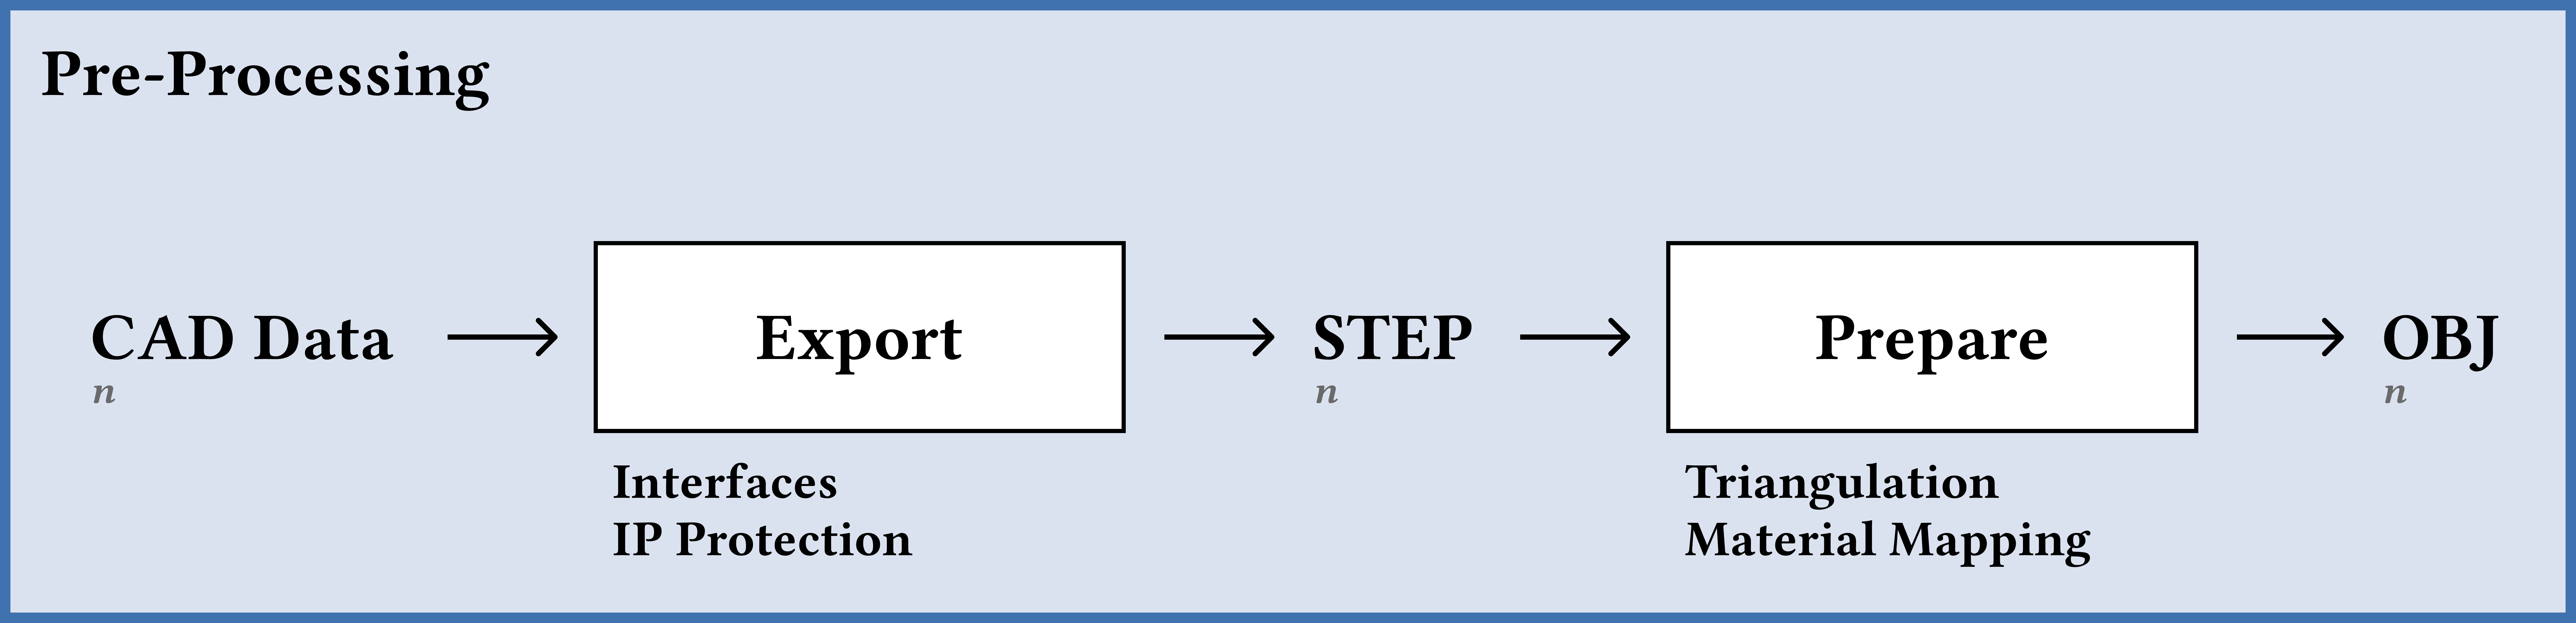
\includegraphics[width=0.9\columnwidth]{resources/cad-pipeline-preprocessing.png}
  \caption{A two-step pre-processing stage is employed for offline as well as real-time rendering pipelines.}
  \label{fig:cad-preprocessing}
\end{figure}

The use of CAD models for designing and manufacturing processes is widespread in industry. These models often contain detailed information about the geometry as well as material properties. Such models are frequently used in mechanical engineering and product design.

Some of the challenges when using CAD models is the lack of detailed material information. Another difficulty can be the complexity of the models. Frequently, the triangulated meshes are too fine-grained. There are approaches, such as algorithms used to generate level of detail (LOD) artifacts, to circumvent this issue.
Another important consideration are intellectual property (IP) rights when using CAD models from production processes. The models may contain proprietary information which should not be disclosed to the end user.
In addition to these factors, the pre-processing step should also define information on what kind of components can be added to the assembly and where they can be attached to. This can be done by providing meta information files containing the information. Alternatively, this can also be represented geometrically within the model by using identifiable shapes to attach components to.

An offline rendering pipeline generates static images of the assembly, which are then displayed in the browser. This means that all possible assemblies need to be rendered and stored upfront. As the number of components increases, the number of possible combinations grows exponentially, which can lead to large amounts of storage and processing power being required, as shown in Figure~\ref{fig:cad-offline}.

\begin{figure}[H]
  
\includegraphics[width=\columnwidth]{resources/cad-pipeline-offline.png}
  \caption{In an offline rendering setup, the number of images grows exponentially. The number of images increases further when offering 360° viewing.}
  \label{fig:cad-offline}
\end{figure}

This is the main benefit of using a real-time rendering pipeline, as illustrated in Figure~\ref{fig:cad-online}. The rendering is done in the browser, which means that the server only needs to provide the geometry and material information in an exchange format such as glTF. This approach is more flexible and can be used for a larger number of configurations. The amount of data to be stored and processed offline grows linearly with the number of components, independent of the number of possible configurations.

\begin{figure}[H]
  
\includegraphics[width=\columnwidth]{resources/cad-pipeline-online.png}
  \caption{A real-time rendering pipeline solely relies on having an adequate model for each component of the assembly. It does not require pre-rendering every possible configuration.}
  \label{fig:cad-online}
\end{figure}

\section{Prior Work}

Work has been conducted in related fields, this includes research into applicability of WebGPU as well as writing web based path tracers using WebGL. However, to the best of my knowledge, no open-source path tracing library using WebGPU has been developed.

\subsection{WebGPU}

Different other applications of WebGPU have been investigated in the past years. One such example is Dynamical.JS, a framework to visualize graphs \cite{dotson2022dynamicaljs}. Another example is RenderCore, a research-oriented rendering engine \cite{Bohak_Kovalskyi_Linev_Mrak_Tadel_Strban_Tadel_Yagil_2024}, or demonstrations on how to use WebGPU for client-side data aggregation \cite{kimmersdorfer2023webgpu}.

Investigation into the performance of WebGPU have been conducted and show that WebGPU can be faster than WebGL \cite{webGPUWebGis, fransson2023performance, CHICKERUR2024919}.
 

\subsection{Web Path Tracers}

There are a variety of path tracers available for the web. Most of them are based on WebGL, a web standard which will be highlighted in the following sections.

The first experiments of using WebGL for path tracing were implemented as early as 2010. One such example is the demo by Evan Wallace showcasing a Cornell Box with basic primitive shapes such as spheres and planes \cite{pathTracerWallace}.

Since then, a variety of open-source implementations for the web have been created.

\subsection{Three.js-based Ray Tracers}

Some of the most widely known path tracers are based on Three.js. Including:

\begin{itemize}
    \item {\texttt{three-gpu-pathtracer}} \cite{ThreeJsPathTracerJohnson}.
    \item{\texttt{Three.js PathTracer}} \cite{ThreeJsPathTracerLoftis}.
    \item {\texttt{dspbr-pt}} \cite{PathTracerDassault}.
  \end{itemize}
